\section{Introduction 10\%}
Nowadays modern vehicles are usually equipped with powerful computers able to read and process data from sensors and cameras. In order to be able to provide the driver useful information fast enough, they should process data also in real time. With the birth and growth of intelligent systems, computer vision is increasingly used in the field of intelligent transport, which includes the subject of this paper: traffic sign recognition. It can be seen as a third eye which concerns a wide area of usages such as advanced driver assisting systems, autonomous driving and vehicle navigations. Other applications are system road surveying, building and maintaining maps of signs, mobile mapping systems, surveillance and self-govern robot navigation systems. These systems are typically based on detecting a region of interest (ROI), in which the traffic sign is located, recognising typical characteristics such as colour and geometric form. These information provide crucial visual details in order to understand the proper driving conditions. For example, they inform about speed limits, drivable lanes, obstacles, temporary situations, roadway access, restrictive areas, etc. Reasons why they are designed to be easily detectable, recognizable and interpretable by humans.
\begin{figure}[h]
	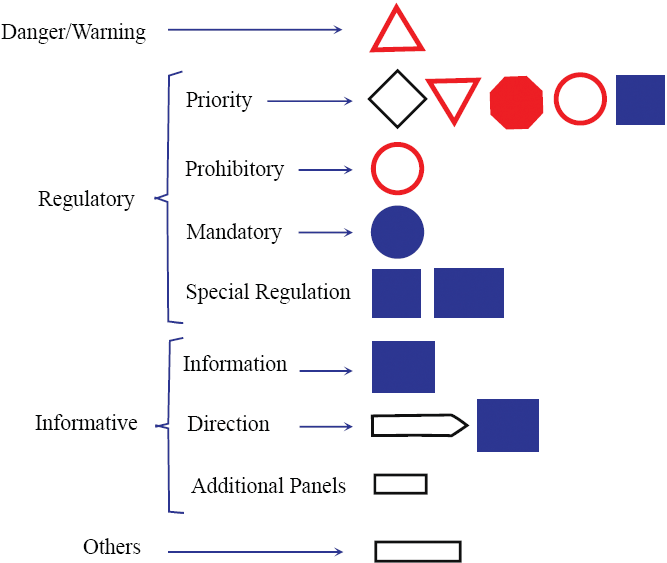
\includegraphics[width=\linewidth]{Res/Immagini/european-traffic-signs.PNG}	
	\caption{European Traffic Sign Categories}
\end{figure}

The application developed includes not only the standard functionality of image processing but also image and video detection and image classification. The idea is to concatenate different processes in order to compute the final labels for each traffic-sign without requiring a big amount of resources. In fact, traffic-sign detectors for large numbers of categories remains a challenging problem.\\ The process starts with the detection stage for the input image or video. This phase exploits the YOLO \cite{yolo} library for object detection which detects the area where a possible traffic sign is located and draws the so-called bounding boxes around it. We chose YOLO because of its main feature of being significantly faster than other framework, trading a bit of accuracy. Once the first step is completed, each object is passed to the classifier which is in charge to find out the correct label for the image. For this purpose we lean on Keras, a deep-learning framework which offers intuitive APIs and fits well for our project.  
%------------------------------------------------------------------------